\section{El método de posición falsa (Regula Falsi)}

El método de la falsa posición pretende conjugar la seguridad del método de la bisección con la rapidez del método de la secante.\newline\newline
Como es denominado \cite{Burden_English}, el término Regula Falsi literalmente “regla falsa” o “posición falsa” (a veces es denominado como el método de adivinar y comprobar. \cite{CS_Web}) se refiera a una técnica en la que se usan resultados que se sabe son falsos, pero de algún modo específico, genera aproximaciones de la misma manera que el método de la secante, pero incluye una prueba para garantizar que la raíz siempre se agrupa entre iteraciones sucesivas, para obtener convergencia a un resultado verdadero. Aunque su convergencia está garantizada, tiene una tasa de convergencia lenta.\newline\newline
Los problemas de posición falsa se pueden encontrar en el papiro Rhind, que data de aproximadamente 1650 a.C.

\begin{figure}[!ht]
    \centering
    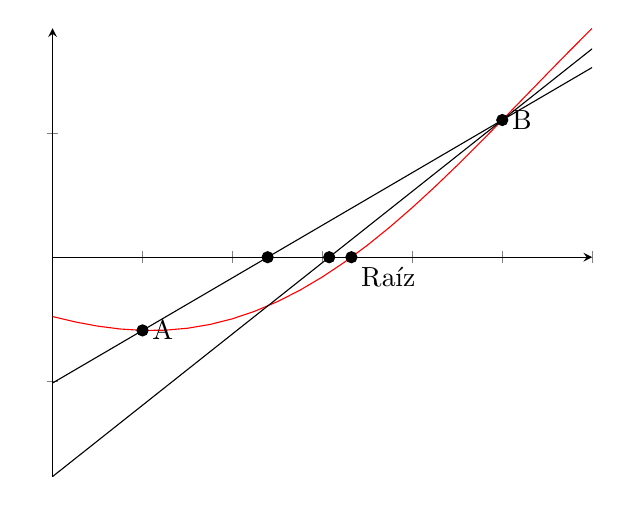
\begin{tikzpicture}
        \begin{axis}[
            axis x line = middle,
            axis y line =  center,
            grid = minor,
            xticklabels={,,},
            yticklabels={,,}
            ]
            \addplot[
                color = red,
                domain=0.5:3.5
                ]{x - 2*sin(deg(x)) - (1 / 2)};
            \addplot[
                color = black,
                domain=0.5:3.5
                ]{(((2.2177 - -1.1829) * (x - 1)) / (3 - 1)) + -1.1829};
            \addplot[
                color = black,
                domain=0.5:3.5
                ]{(((2.2177 - -0.788714) * (x - 1.6957)) / (3 - 1.6957)) + -0.788714};
            \filldraw[black] (2.1613,-0.0000037) circle (2pt) node[anchor=north west]{Raíz};
            \filldraw[black] (1, -1.1829) circle (2pt) node[anchor=west]{A};
            \filldraw[black] (3, 2.2177) circle (2pt) node[anchor=west]{B};
            \filldraw[black] (1.6957, 0) circle (2pt) node[anchor=west]{};
            \filldraw[black] (2.0378, 0) circle (2pt) node[anchor=west]{};
        \end{axis}
    \end{tikzpicture}
    \caption{Gráfica del método de la falsa posición}
    \label{regula_grap_ej1}
\end{figure}